\section{Les sources du Big Data :}
Pour réussir avec le Big Data, il est important que les entreprises disposent du savoir-faire pour passer en revue les différentes sources de données disponibles et classer en conséquence leur convivialité et leur pertinence. Deux classifications des sources du Big Data sont données dans ce qui suit :

\begin{enumerate}
\item Selon qu'elles soient internes ou externe à l'entreprise.
\item Selon leur provenance.
\end{enumerate}

\subsection{Les données internes ou externes à l'entreprise}
Les données sont internes si une entreprise les génère, les possède et les contrôle.

\textbf{Exemple :}
\begin{itemize}[label=\textbullet]
\item Module ERP d'entreprise.
\item Capteurs, contrôleurs.
\item Centres d'appels internes.
\item Journaux de site Web.
\end{itemize}

Les données externes sont des données publiques ou des données générées en dehors de l'entreprise ; en conséquence, la société ne la possède ni ne la contrôle. Exemple :
\begin{itemize}[label=\textbullet]
\item Médias sociaux.
\item Statistiques officielles.
\item Ensembles de données accessibles au public pour l'apprentissage automatique.
\end{itemize}

\subsection{Les sources du Big Data selon leur provenances :}
Les données les plus volumineuses sont utilisées aujourd'hui par les organisations et les entreprises dans le seul but d'effectuer des analyses. Toutefois, avant de pouvoir extraire des informations et des renseignements précieux à partir de données importantes, ces dernières doivent connaître plusieurs sources de données importantes. Les données, comme nous le savons, sont massives et existent sous diverses formes. Si elles ne sont pas bien classées ou si elles ne proviennent pas d'une source sure, elles peuvent finir par faire perdre du temps et des ressources précieuses. Afin de réussir avec les données volumineuses, il est important que les entreprises aient le savoir-faire nécessaire pour faire le tri entre les différentes sources de données disponibles et classer en conséquence leur utilité et leur pertinence.

\begin{figure}[h]
	\centering
    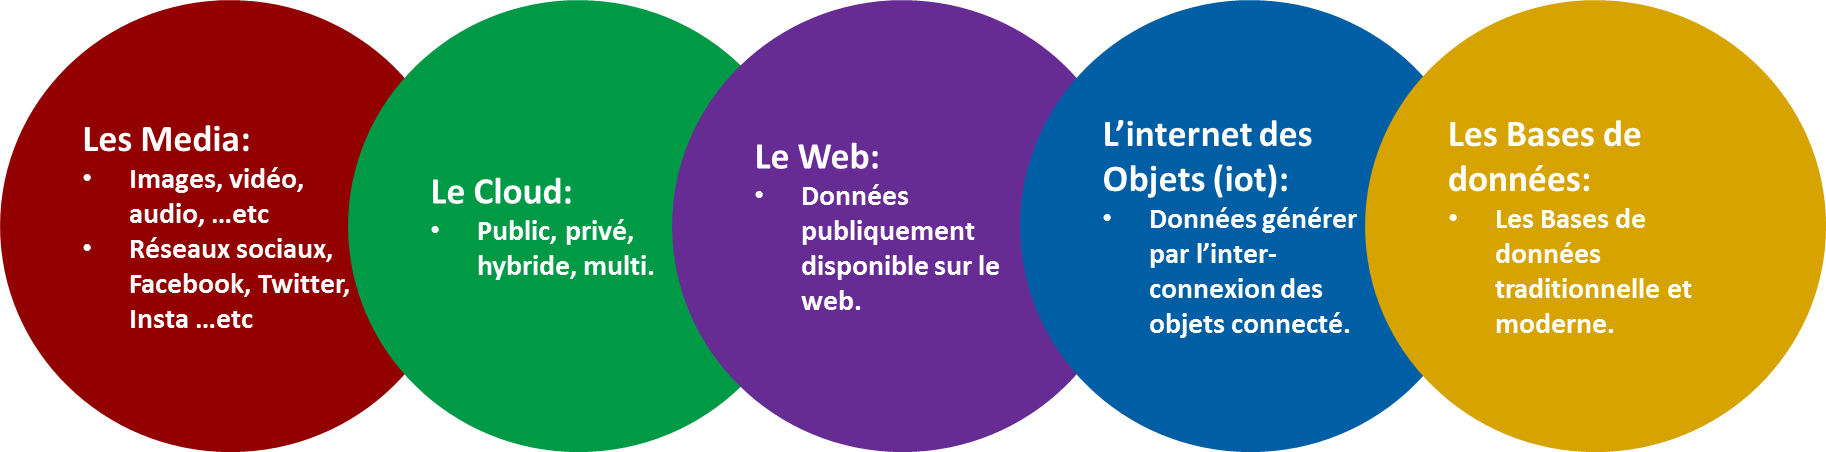
\includegraphics[scale=0.5]{img/part1/1.7}
    \caption{Les sources du Big Data}
\end{figure}

\subsubsection{Les médias :}
Les médias sont la source la plus populaire de méga données, car ils fournissent des informations précieuses sur les préférences des consommateurs et l'évolution des tendances. Ces données sociales proviennent des mentions J'aime, des tweets et des retweets, des commentaires, des téléchargements de vidéos et des médias généraux qui sont téléchargés et partagés via les plateformes de médias sociaux préférées au monde. Ce type de données fournit des informations inestimables sur le comportement et le sentiment des consommateurs et peut être extrêmement influent dans les analyses marketing.

\textit{\textbf{Exemple :}Les médias comprennent les médias sociaux et les plates-formes interactives, telles que Google, Facebook, Twitter, YouTube, Instagram, ainsi que des supports génériques tels que des images, des vidéos, des audio et des podcasts qui fournissent des informations sur l'interaction utilisateur.}

\subsubsection{Le Cloud :}
Aujourd'hui, avec la croissance accélérée du volume de données utilisé par les applications, de nombreuses organisations ont déplacé leurs données vers des serveurs Cloud pour fournir des services évolutifs,  ables et hautement disponibles [12].

Le stockage Cloud héberge des données structurées et non structurées et fournit aux entreprises des informations en temps réel et des informations à la demande. Le principal attribut du Cloud computing est sa flexibilité et son évolutivité. Comme les méga données peuvent être stockées et sourcées sur des Clouds publics ou privés, via des réseaux et des serveurs, le Cloud constitue une source de données efficace et économique car les ressources sont fournis à la demande et on ne paye que les ressources utilisées.

\subsubsection{Le Web :}
Le Web public constitue une source répandu et facilement accessible pour le Big Data. Les données sur le Web ou “Internet“ sont généralement disponibles pour les particuliers et les entreprises. De plus, des services Web tels que Wikipédia fournissent des informations gratuites et rapides à tout le monde. Le Web public est également une autre bonne source de données sociales, et des outils comme Google Trends peuvent être utilisés à bon escient pour augmenter le volume de données.

L'énormité du Web garantit sa polyvalence et est particulièrement bénéfique pour les start-ups et les PME, car elles n'ont pas à attendre pour développer leur propre infrastructure et référentiels de Big Data avant de pouvoir tirer parti du Big Data.

\subsubsection{L'Internet Des Objets (IoT) :}
Les données machine sont définies comme des informations générées par des équipements industriels, des capteurs installés dans des machines et même des journaux Web qui suivent le comportement de l'utilisateur. En logistique, il peut s'agir de capteurs qui servent à la traçabilité des biens pour la gestion des stocks et les acheminements.

En domotique, l'IoT recouvre tous les appareils électroménagers communicants, les capteurs, les compteurs intelligents et systèmes de sécurité connectés des appareils de type box domotique. Le phénomène IoT est également très visible dans le domaine de la santé et du bien-être avec le développement des montres connectées, des bracelets connectés et d'autres capteurs surveillant des constantes vitales.

\textit{\textbf{Exemple :} En Tennis, la marque Zepp propose un système de capteur connecté qui analyse vos performances sur le terrain. Il suffit de fixer le capteur sur le manche de n'importe quelle raquette de tennis et de se mouvoir pour obtenir un retour d'information instantané sur iPhone, iPad ou appareil Android.}

\subsubsection{Les bases de données :}
Les entreprises préfèrent aujourd'hui utiliser une fusion de bases de données traditionnelles et modernes pour acquérir des méga données pertinentes. Cela permet d'ouvrir la voie à un modèle de données hybride avec un faible coût d'investissement. De plus, ces bases de données sont également déployées à plusieurs  ns de Business Intelligence. Le processus d'extraction et d'analyse de données parmi de vastes sources de méga données est un processus complexe qui peut être frustrant. Ces complications peuvent être résolues si les organisations englobent toutes les considérations nécessaires des méga données, et prennent en compte les sources de données pertinentes et les déploient d'une manière bien adaptée à leurs objectifs organisationnels.

\textit{\textbf{Exemple :} Les bases de données les plus populaires Microsoft SQL Server, MongoDB, Oracle, MySQL et IBM Db2 ...etc.}

